% !TEX root = main.tex
\chapter{Real time decoder}
\label{cha:decoder}

This chapter describes the implementation
of the new {\it OnlLatgenFasterDecoder}\/ and 
the modification of an online speech parametrisation and feature transformations.

We limited our task, so it fits our requirements for real time decoding
in our \ac{SDS} Alex.
We need a real time decoder with sufficient accuracy,
which does not apply any speaker adaptive transformations.
We strongly prefer n-best list or lattice output formats over one-best hypothesis.
In addition, we require latency under 0.2 seconds after the end of user speech.

We also wanted to reuse existing code as much as possible,
so the decoder will benefit from constant development on Kaldi toolkit.
As a bonus of the minimal changes we can compare our {\it OnlLatgenFasterDecoder}\/ 
with {\it LatgenFasterDecoder}\/ which is used through binary executable {\it gmm-latgen-faster}.
Correctly setup, the decoders produce exactly the same results.




\todo{dej do evaluation, ze rozeberes nejenom presnost 
ale i rychlosty dekoderu, a rohodnes ktery dekoder z Kaldi je vhodny a jake nastaveni potrebuje pro RT performance.}

\todo{decoding lattices and normal outputs -- describe again the problems}

\todo{dat tam analyza -> future improvements}

\todo{udelat real time experiment }

\section{Online pre-processing} 
\label{sec:onl_preprocess}

\begin{figure}[!ph]
    \begin{center}
        % Graphic for TeX using PGF
% Title: /home/ondra/Diagram1.dia
% Creator: Dia v0.97.2
% CreationDate: Thu Aug  1 08:02:11 2013
% For: ondra
% \usepackage{tikz}
% The following commands are not supported in PSTricks at present
% We define them conditionally, so when they are implemented,
% this pgf file will use them.
\ifx\du\undefined
  \newlength{\du}
\fi
\setlength{\du}{15\unitlength}
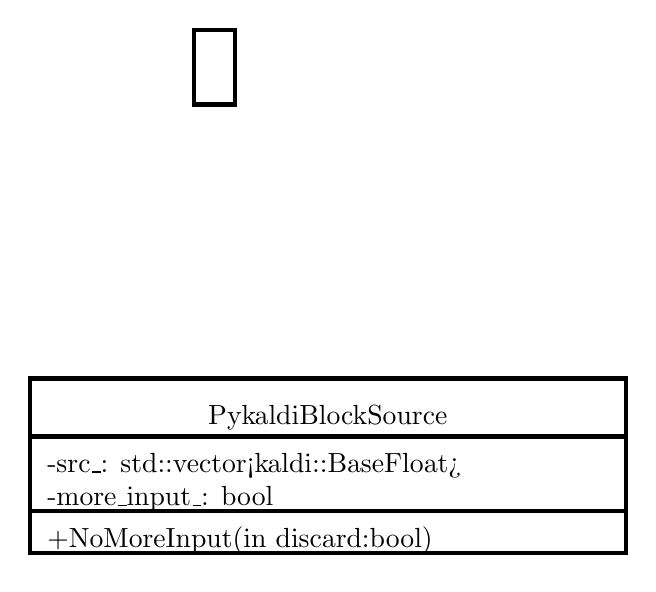
\begin{tikzpicture}
\pgftransformxscale{1.000000}
\pgftransformyscale{-1.000000}
\definecolor{dialinecolor}{rgb}{0.000000, 0.000000, 0.000000}
\pgfsetstrokecolor{dialinecolor}
\definecolor{dialinecolor}{rgb}{1.000000, 1.000000, 1.000000}
\pgfsetfillcolor{dialinecolor}
\pgfsetlinewidth{0.100000\du}
\pgfsetdash{}{0pt}
\definecolor{dialinecolor}{rgb}{1.000000, 1.000000, 1.000000}
\pgfsetfillcolor{dialinecolor}
\fill (13.250000\du,6.900000\du)--(13.250000\du,8.700000\du)--(14.250000\du,8.700000\du)--(14.250000\du,6.900000\du)--cycle;
\definecolor{dialinecolor}{rgb}{0.000000, 0.000000, 0.000000}
\pgfsetstrokecolor{dialinecolor}
\draw (13.250000\du,6.900000\du)--(13.250000\du,8.700000\du)--(14.250000\du,8.700000\du)--(14.250000\du,6.900000\du)--cycle;
% setfont left to latex
\definecolor{dialinecolor}{rgb}{0.000000, 0.000000, 0.000000}
\pgfsetstrokecolor{dialinecolor}
\node at (13.750000\du,7.995000\du){};
% setfont left to latex
\pgfsetlinewidth{0.050000\du}
\definecolor{dialinecolor}{rgb}{0.000000, 0.000000, 0.000000}
\pgfsetstrokecolor{dialinecolor}
\draw (13.750000\du,8.147500\du)--(13.750000\du,8.147500\du);
\pgfsetlinewidth{0.100000\du}
\pgfsetdash{}{0pt}
\definecolor{dialinecolor}{rgb}{1.000000, 1.000000, 1.000000}
\pgfsetfillcolor{dialinecolor}
\fill (9.300000\du,15.300000\du)--(9.300000\du,16.700000\du)--(23.660000\du,16.700000\du)--(23.660000\du,15.300000\du)--cycle;
\definecolor{dialinecolor}{rgb}{0.000000, 0.000000, 0.000000}
\pgfsetstrokecolor{dialinecolor}
\draw (9.300000\du,15.300000\du)--(9.300000\du,16.700000\du)--(23.660000\du,16.700000\du)--(23.660000\du,15.300000\du)--cycle;
% setfont left to latex
\definecolor{dialinecolor}{rgb}{0.000000, 0.000000, 0.000000}
\pgfsetstrokecolor{dialinecolor}
\node at (16.480000\du,16.250000\du){PykaldiBlockSource};
\definecolor{dialinecolor}{rgb}{1.000000, 1.000000, 1.000000}
\pgfsetfillcolor{dialinecolor}
\fill (9.300000\du,16.700000\du)--(9.300000\du,18.500000\du)--(23.660000\du,18.500000\du)--(23.660000\du,16.700000\du)--cycle;
\definecolor{dialinecolor}{rgb}{0.000000, 0.000000, 0.000000}
\pgfsetstrokecolor{dialinecolor}
\draw (9.300000\du,16.700000\du)--(9.300000\du,18.500000\du)--(23.660000\du,18.500000\du)--(23.660000\du,16.700000\du)--cycle;
% setfont left to latex
\definecolor{dialinecolor}{rgb}{0.000000, 0.000000, 0.000000}
\pgfsetstrokecolor{dialinecolor}
\node[anchor=west] at (9.450000\du,17.400000\du){-src\_: std::vector<kaldi::BaseFloat>};
% setfont left to latex
\definecolor{dialinecolor}{rgb}{0.000000, 0.000000, 0.000000}
\pgfsetstrokecolor{dialinecolor}
\node[anchor=west] at (9.450000\du,18.200000\du){-more\_input\_: bool};
\definecolor{dialinecolor}{rgb}{1.000000, 1.000000, 1.000000}
\pgfsetfillcolor{dialinecolor}
\fill (9.300000\du,18.500000\du)--(9.300000\du,19.500000\du)--(23.660000\du,19.500000\du)--(23.660000\du,18.500000\du)--cycle;
\definecolor{dialinecolor}{rgb}{0.000000, 0.000000, 0.000000}
\pgfsetstrokecolor{dialinecolor}
\draw (9.300000\du,18.500000\du)--(9.300000\du,19.500000\du)--(23.660000\du,19.500000\du)--(23.660000\du,18.500000\du)--cycle;
% setfont left to latex
\definecolor{dialinecolor}{rgb}{0.000000, 0.000000, 0.000000}
\pgfsetstrokecolor{dialinecolor}
\node[anchor=west] at (9.450000\du,19.200000\du){+NoMoreInput(in discard:bool)};
\end{tikzpicture}

    \caption{Aggregation of classes for serial input processing}
    \label{fig:classes} 
    \end{center}
\end{figure}


\section{online decoder interface} 
\label{sec:improve}

\todo{How I split the LatgenFasterDecoder}

\todo{desscribe the behaviour of all functions especially the decode function}


\section{Post-processing the state lattice}
\label{sec:postprocess}

\todo{How I converted the state lattice to word posterior lattice}

\todo{The trick with discarding alignments}

\section{Objected oriented interface to speech recognition}
\label{sec:ooi}

\todo{How I wrapped up the code instead of creating a binary executable}

\section{The setup for real-time decoding}

\todo{WER - with equivalent setup as gmm-latgen-faster, describe the relation ship. Maybe reference pykaldi/binutils}

\todo{The WER evaluation in SDS setup described in next chapter}

\todo{Which parameters influence decoding, which setup on which machine we use it}

\todo{profiling -cpu, spent time in which methods, memory profiling}

% \section[Comparison of real time decoders]{Comparison of real time decoders in Alex dialog system} 
% \label{sec:comparison_of_real_time_decoders_in_alex_dialog_system}
% Further, in this section we will briefly compare the main qualities of used decoders.
% Namely, we will compare: 
% \begin{itemize}
%     \item Kaldi online decoder - Acoustic models were trained by training scripts for Kaldi described at~\ref{cha:models}.
%     \item HDecode - HDecode is \ac{HTK} decoder and it decodes from acoustic models trained by \ac{HTK}.
% \end{itemize}


\section{Summary}
\label{sec:onl_summary}
The {\it OnlLatgenFasterDecoder}\/ is able to perform real-time decoding.
Its parameters for real-time decoding, 
can be setup based on its reference batch decoder {\it LatgenFasterDecoder}\/ used through {\it gmm-latgen-faster}\/ executable.

The minimal interface for speech parametrisation and feature transformations is not usable in general case,
but works very well for the implemented setup.
Our setup support \ac{MFCC} speech parametrisation, $\Delta+\Delta-\Delta$ or \ac{LDA} transformation, with
classic Viterbi trained \ac{AM} or \ac{AM} trained using \ac{bMMI}.
The setup yields the best results for non-speaker adaptive methods.

\subsection{Future improvements}
\label{sub:onl_future}
As described, we support a narrow range of feature transformation,
so it would be natural to implement more complicated online interface,
which could support more feature transformations, 
which are available in Kaldi toolkit for batch mode. 

In next work, we would like to focus on acoustic modeling with \acl{DNN}.
The \ac{DNN} provide more accurate acoustic probabilities, 
which should lead to faster beam search,
because the search is more informed.\cite{TODO_DNN} 
We see the challenge in implementation of \acl{DNN} evaluation in real time, probably using \ac{GPU}.
Note that the Kaldi toolkit already support \ac{DNN} training and evaluation.
\todo{Write Karel Vesely and ask him how fast is the evaluation}
